\documentclass{article}\usepackage{float}

% Language setting
% Replace `english' with e.g. `spanish' to change the document language
\usepackage[english]{babel}

% Set page size and margins
% Replace `letterpaper' with `a4paper' for UK/EU standard size
\usepackage[letterpaper,top=2cm,bottom=2cm,left=3cm,right=3cm,marginparwidth=1.75cm]{geometry}

% Useful packages
\usepackage{amsmath}
\usepackage{booktabs} 
\usepackage{graphicx}
\usepackage{tabularx}
\usepackage{longtable} 
\usepackage[colorlinks=true, allcolors=blue]{hyperref}

\title{Klasifikasi Akronim dan Ekspansinya dengan Algorithma Supervised Learning dan BERT}
\author{Najwan Yusnianda \\ NIM: 2408207010029}
\date{}

\begin{document}
\maketitle



\section{Introduction}

Selama beberapa dekade terakhir, identifikasi pasangan akronim dan perluasannya dari korpus teks besar telah menjadi topik penelitian yang menarik perhatian luas, terutama dalam bidang text mining, ekstraksi entitas, dan pencarian informasi. Akronim, sebagai bentuk singkatan dari frasa atau istilah panjang, sering digunakan dalam berbagai domain. Namun, penggunaan akronim yang tidak konsisten atau ambigu dapat menimbulkan tantangan dalam pemrosesan teks otomatis, terutama ketika mencoba memahami makna sebenarnya dari suatu dokumen atau teks.

Tantangan utama dalam identifikasi akronim adalah menentukan pasangan yang tepat antara akronim dan ekspansinya, terutama dalam korpus yang besar dan beragam. Proses ini memerlukan pendekatan yang canggih untuk memastikan akurasi dan keandalan dalam ekstraksi informasi.
Salah satu penelitian yang signifikan dilakukan oleh Taufik et al. \cite{ref1}, yang memperkenalkan delapan fitur vektor untuk menggambarkan hubungan antara akronim dan ekspansinya. Fitur-fitur ini dirancang untuk menangkap karakteristik dari pasangan akronim dan ekspansi, sehingga memungkinkan model machine learning untuk mendapatkan akurasi yang tinggi dan optimal dalam klasifikasi. Penelitian ini menunjukkan bahwa pendekatan berbasis fitur yang dirancang dengan baik dapat menjadi solusi efektif untuk masalah identifikasi akronim.

Namun, dengan kemajuan pesat dalam bidang pemrosesan bahasa alami (Natural Language Processing/NLP), pendekatan berbasis deep learning, khususnya model berbasis transformer seperti BERT (Bidirectional Encoder Representations from Transformers), telah menunjukkan kinerja yang luar biasa dalam berbagai tugas NLP, termasuk klasifikasi teks dan ekstraksi informasi. Model ini mampu menangkap konteks dan makna kata secara lebih mendalam, sehingga berpotensi meningkatkan akurasi dalam identifikasi pasangan akronim-ekspansi.

Penelitian ini bertujuan untuk mengeksplorasi dan membandingkan dua pendekatan utama dalam identifikasi pasangan akronim-ekspansi: metode klasifikasi supervised learning dan metode klasifikasi deep learning berbasis transformer menggunakan BERT. Dengan membandingkan kedua pendekatan ini, penelitian ini diharapkan dapat memberikan wawasan tentang metode mana yang lebih efektif dalam menyelesaikan permasalahan akronim dan ekspansinya, serta memberikan rekomendasi untuk pengembangan model yang lebih baik di masa depan.





\section{Methodology }

\subsection{Dataset}

Dataset yang digunakan dalam penelitian ini berasal dari dataacro \cite{ref1} berupa teks yang terdiri dari pasangan akronim dan ekspansinya serta label(-1 dan 1) serta 8 fitur hasil dari ekstraksi fitur pasangan akronim yang telah diekstraksi. Dataset ini terdiri dari training set (4000 sampel) dengan testing set (1099 sampel). Berikut adalah beberapa contoh training set:

\begin{verbatim}
BUMD=>Usaha Milik -1 1:0.918 2:1 3:-0.667 4:0 5:1 6:0.5 7:0 8:0.393
TNI=>meminjam senjata dari oknum -1 1:1 2:0.5 3:-2 4:0 5:0.75 6:0 7:0 8:0.036
PKI=>Panitia Pengawas -1 1:0.971 2:1 3:-1 4:0.5 5:1 6:0.333 7:0 8:0.401
\end{verbatim}

Data tersebut selanjutnya dilakukan proses preprocessing dan mengubahnya menjadi 2 bagian untuk supervised learning dan untuk Deep Learning Berbasis Transformer.
Pada Model supervised learning, Data yang digunakan berupa fitur -fitur yang telah diekstrak seperti yang dijelaskan sebelumnya. rincian fitur-fitur tersebut adalah sebagai berikut:

\begin{itemize}
    \item \textbf{Fitur 1}: Korelasi antara jumlah total karakter dalam akronim dan total jumlah kata dalam ekspansi.
    \item \textbf{Fitur 2}: Jumlah kata dalam ekspansi yang menggunakan huruf besar pada awal kata.
    \item \textbf{Fitur 3}: Penimbang kecocokan huruf-huruf dalam akronim dan ekspansi/kepanjangannya, tidak termasuk kata sambung.
    \item \textbf{Fitur 4}: Penimbang korelasi antara huruf pertama dan terakhir dari akronim.
    \item \textbf{Fitur 5}: Nilai penalti kepada akronim yang mengandung banyak preposisi (kata depan) dan konjungsi (kata penghubung).
    \item \textbf{Fitur 6}: Rasio kecocokan yang tepat antara karakter dalam ekspansi dan karakter dalam akronim.
    \item \textbf{Fitur 7}: Nilai pembeda antara rasio kecocokan yang akurat (Fitur 6) dan rasio yang tidak akurat.
    \item \textbf{Fitur 8}: Rata-rata dari Fitur 1 hingga Fitur 7.
\end{itemize} 

\begin{table}
\centering
\begin{tabular}{r|*{9}{l}}
Index & F1 & F2 & F3 & F4 & F5 & F6 & F7 & F8 & label \\ \midrule
0 & 0.918 & 1.000 & -0.667 & 0.000 & 1.000 & 0.500 & 0.000 & 0.393 & 0 \\
1 & 1.000 & 0.500 & -2.000 & 0.000 & 0.750 & 0.000 & 0.000 & 0.036 & 0 \\
2 & 0.971 & 1.000 & -1.000 & 0.500 & 1.000 & 0.333 & 0.000 & 0.401 & 0 \\
3 & 1.000 & 0.750 & -2.000 & 0.000 & 1.000 & 1.000 & 1.000 & 0.393 & 0 \\
4 & 0.971 & 0.667 & -2.500 & 0.000 & 1.000 & 0.000 & 0.000 & 0.020 & 0 \\
\bottomrule
\end{tabular}
\caption{\label{tab:data} Sampel dataset yang digunakan untuk supervised learning.}
\end{table}



Sedangkan pada model deep learning berbasis transformer, data yang digunakan berupa teks yang belum diekstrak. Hali ini karena Transformer khususnya BERT mempunyai metode embedding tersendiri untuk mengubah teks menjadi fitur vektor sehingga tidak perlu ekstraksi fitur.

\begin{table}
\centering
\begin{tabular}{r|l|r}
\toprule
Index & Fitur teks & Label \\ \midrule
0 & BUMD $\rightarrow$ Usaha Milik & 0 \\
1 & TNI $\rightarrow$ meminjam senjata dari oknum & 0 \\
2 & PKI $\rightarrow$ Panitia Pengawas & 0 \\
3 & MA $\rightarrow$ putusan Mahkamah & 0 \\
4 & TI $\rightarrow$ com Mati body & 0 \\ \bottomrule
\end{tabular}
\caption{\label{tab:text_features}Sampel dataset yang digunakan untuk BERT.}
\end{table}

\subsection{Descriptive Analysis }

Pada gambar \ref{fig:Dist_Feature} menunjukan  nilai antar fitur memiliki variasi yang beragam. Sebagian besar fitur, seperti F1, F2, F4, F5, dan F7, menunjukkan distribusi yang cenderung berada pada nilai mendekati 0 atau 1. Fitur lainnya, seperti F3, F6, dan F8, memiliki distribusi yang lebih tersebar, menunjukkan adanya variasi yang lebih merata dalam fitur-fitur tersebut. Hal ini dapat memberikan gambaran penting terkait s berkontribusi pada model yang akan dibangun.

\begin{figure}
\centering
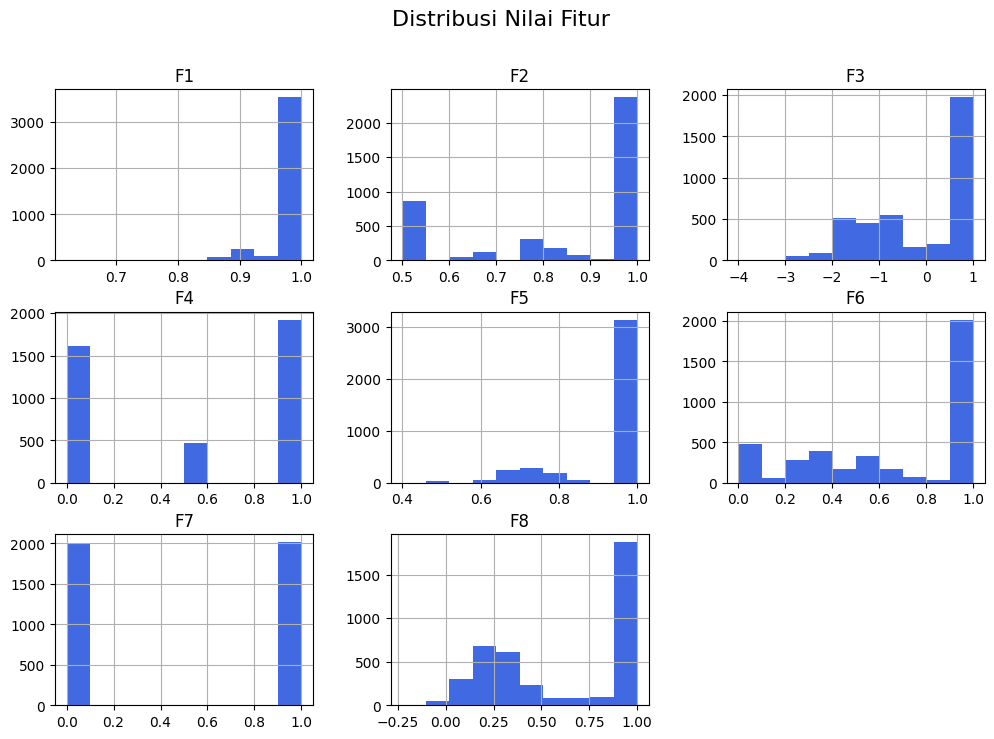
\includegraphics[width=1\linewidth]{img/dist_fitur.png}
\caption{\label{fig:Dist_Feature}Distribusi nilai fitur-fitur akronim dan ekspansinya dalam training set}
\end{figure}

Selanjutnya Distribusi Training sampel pada gambar \ref{fig:Dist_Label} memiliki jumlah sampel yang sama untuk setiap kelas yaitu kelas 0 dan 1 yaitu 2000 sample untuk masing -masing kelas. Kelas 0 merupakan kelas yang sebelumnya bernilai -1 sebelum dilakukan preprocessing untuk memudahkan pada saat pelatihan model.


\begin{figure}
\centering
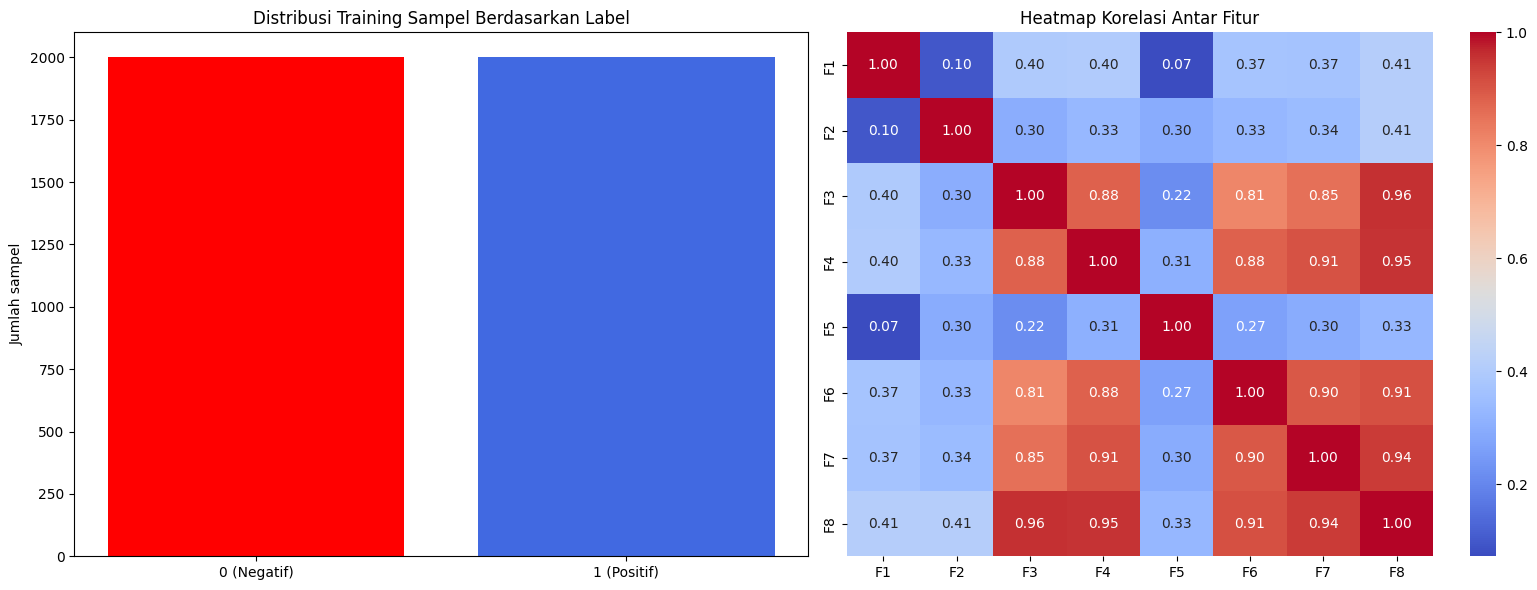
\includegraphics[width=1\linewidth]{img/dist_label.png}
\caption{\label{fig:Dist_Label}Distribusi nilai kelas dan korelasi antar fitur pada training set}
\end{figure}


Analisis korelasi antar fitur 1 hingga 8 menunjukkan hubungan yang signifikan, dengan beberapa fitur memiliki korelasi yang sangat tinggi. Secara spesifik, fitur F3, F4, F6, F7, dan F8 menunjukkan korelasi yang sangat kuat satu sama lain, dengan koefisien korelasi mencapai hampir 1, mengindikasikan adanya ketergantungan yang tinggi antar fitur tersebut. Sebaliknya, fitur F1 dan F2 memiliki korelasi yang relatif rendah dengan sebagian besar fitur lainnya. Fitur F5 juga menunjukkan korelasi yang lebih rendah dibandingkan dengan kelompok fitur yang berkorelasi tinggi tersebut. Hal ini menunjukkan bahwa meskipun ada kelompok fitur yang memiliki dependensi yang tinggi,namun masih terdapat fitur-fitur independen yang dapat memberikan informasi tambahan dan berpotensi meningkatkan akurasi model dalam analisis data akronim dan ekspansinya. 


\subsection{Model and Algorithms }
Penelitian ini menggunakan model dan algoritma supervised learning dengan memanfaatkan delapan fitur tersebut untuk menemukan model terbaik. Model-model tersebut kemudian dibandingkan dengan model berbasis Transformer, yaitu BERT (Bidirectional Encoder Representations from Transformers). Model supervised learning yang digunakan adalah sebagai berikut:
\begin{itemize}
    \item \textbf{Support Vector Machine (SVM)}: Algoritma yang bekerja dengan menemukan hyperplane terbaik untuk memisahkan kelas dalam ruang fitur.
    \item \textbf{K-Nearest Neighbor (KNN)}: Algoritma yang mengklasifikasikan data berdasarkan kedekatan jarak dengan tetangga terdekatnya.
    \item \textbf{Naive Bayes}: Algoritma probabilistik yang didasarkan pada teorema Bayes dengan asumsi independensi antar fitur.
    \item \textbf{Decision Tree}: Algoritma yang memodelkan keputusan dalam bentuk pohon dengan aturan-aturan berbasis fitur.
\end{itemize}

Selanjutnya, model berbasis \textbf{BERT} digunakan sebagai pembanding. Model ini memanfaatkan arsitektur transformer untuk menangkap konteks dari kata secara lebih mendalam melalui mekanisme self-attention, sehingga mampu menghasilkan representasi vektor yang kaya akan informasi semantik. Dengan pendekatan ini, BERT dapat memberikan hasil yang lebih baik dalam klasifikasi teks.

\subsection{Experimental Setup }

Eksperimen dilakukan menggunakan Python dengan framework Scikit-Learn untuk supervised learning dan PyTorch untuk fine-tuning BERT.

\subsubsection*{Tahapan untuk Supervised Learning}
Tahapan supervised learning adalah sebagai berikut:
\begin{itemize}
    \item \textbf{Penyiapan Dataset}: Dataset yang digunakan merupakan data akronim dan ekspansinya yang telah dilakukan ekstraksi fitur menjadi delapan fitur penting (F1 hingga F8).
    \item \textbf{Tuning Hyperparameter}: Dilakukan dengan \textit{GridSearchCV} untuk menentukan hyperparameter terbaik.
    \item \textbf{Pelatihan Model}: Model dilatih dengan 4000 sampel training set dan 1099 sampel testing set.
    \item \textbf{Evaluasi Model}: Selanjutnya, setiap model dievaluasi menggunakan metrik evaluasi yang telah ditentukan.
\end{itemize}

\subsubsection*{Tahapan untuk BERT}
Tahapan untuk deep learning berbasis transformer dengan BERT adalah sebagai berikut:
\begin{itemize}
    \item \textbf{Penyiapan Dataset}: Dataset yang digunakan terdiri dari fitur `akronim=>ekspansi` serta label yang perlu dilakukan preprocessing menggunakan tokenizer dari BERT. Data kemudian disimpan dalam dataset custom dalam bentuk tensor agar dapat dilatih dalam PyTorch.
    \item \textbf{Inisiasi Model dan Bert Tokenizer}: Mengimpor model BERT (pre-trained) sebelumnya dari Hugging Face dan melakukan tokenisasi.
    \item \textbf{Menyiapkan Trainer dan Fine-Tuning}: Model pre-trained BERT dilatih dengan 4000 sampel training set.
    \item \textbf{Evaluasi Model}: Selanjutnya, model dievaluasi menggunakan metrik evaluasi yang telah ditentukan.
\end{itemize}

\subsection{Evaluation Metric}

Metrik evaluasi utama yang digunakan adalah F1-Score, didukung dengan True Positive (TP), False Positive (FP), False Negative (FN) dan True Negative (TN). Rincian Metrik yang digunakan adalah sebagai berikut:
\begin{itemize}
    \item \textbf{F1-score}: \\
    F1-score merupakan harmonic mean antara precision dan recall. Metrik ini berguna untuk menyeimbangkan antara precision dan recall, terutama pada dataset yang tidak seimbang.
    \[
    F1 = \frac{2 \times \text{Precision} \times \text{Recall}}{\text{Precision} + \text{Recall}}
    \]
    
    \item \textbf{Precision}: \\
    Precision mengukur ketepatan model dalam mengklasifikasikan positif, dihitung sebagai rasio antara prediksi positif yang benar dengan total prediksi positif.
    \[
    \text{Precision} = \frac{TP}{TP + FP}
    \]
    
    \item \textbf{Recall (Sensitivity)}: \\
    Recall mengukur sejauh mana model dapat menemukan seluruh sampel positif yang sebenarnya.
    \[
    \text{Recall} = \frac{TP}{TP + FN}
    \]
    
    \item \textbf{True Positive (TP)}:
    Jumlah sampel positif yang diklasifikasikan dengan benar sebagai positif.
    
    \item \textbf{False Positive (FP)}:
    Jumlah sampel negatif yang salah diklasifikasikan sebagai positif.
    
    \item \textbf{False Negative (FN)}: 
    Jumlah sampel positif yang salah diklasifikasikan sebagai negatif.
    
    \item \textbf{True Negative (TN)}:
    Jumlah sampel negatif yang diklasifikasikan dengan benar sebagai negatif.
\end{itemize}

\section{Results and Discussion}

Serangkaian eksperimen telah dilakukan untuk mengevaluasi kinerja model supervised learning dan model deep learning berbasis transformer BERT. Dalam tahapan pelatihan model, optimasi hyperparameter pada model - model Supervised learning dilakukan melalui metode Grid Search yang diimplementasikan dengan 10-fold cross-validation untuk mendapatkan performa optimal dari tiap model. Hyperparameter terbaik yang berhasil diidentifikasi untuk setiap model disajikan dalam Tabel \ref{tab:Gridsearch_training}

\begin{table}[ht!]
\centering

\begin{tabular}{llll}
\toprule
Model & Grid Search & Parameter Terbaik \\
\midrule
SVM & C: [100.0, 500.0, 1000] & C: 500 \\
 & Gamma: [0.1, 0.2, 0.3, 0.4, 0.5] & Gamma: 0.2 \\
 & Degree: [2, 3, 4] & Degree: 2 \\
 & Kernel: ['linear', 'rbf', 'poly'] & Kernel: poly \\
\midrule
KNN & n\_neighbor: [2, 3, 4, 5, 6, 7, 8, 9] & n\_neighbor: 9 \\
\midrule
Naive Bayes & - & - \\
\midrule
Decision Tree & max\_depth: [3, 5, 10, None] & max\_depth: 3 \\
 & min\_samples\_split: [2, 5, 10] & min\_samples\_split: 2 \\
 & min\_samples\_leaf: [1, 2, 5] & min\_samples\_leaf: 1 \\
 & criterion: ["gini", "entropy"] & criterion: 'gini' \\
\bottomrule

\end{tabular}
\caption{\label{tab:Gridsearch_training} Pencarian grid dan hyperparameter terbaik pada model supervised learning.}
\end{table}

Evaluasi hasil pelatihan yang telah dilakukan dibagi menjadi dua bagian yaitu evaluasi pada Training set dan evaluasi pada Testing set berdasarkan metriks yang telah ditentukan


\subsection{Evaluasi Training Model}



\begin{table}[h!]
\centering
\begin{tabular}{r|l|l|r|r|r|r}
\toprule
No & Model                        & Confusion Matrix          & TP   & FP   & FN   & TN   \\ \midrule
0  & Support Vector Machine (SVM) & [[1961, 39], [13, 1987]]  & 1987 & 39   & 13   & 1961 \\
1  & K-Nearest Neighbor (KNN)     & [[1967, 33], [1232, 768]] & 768  & 33   & 1232 & 1967 \\
2  & Naive Bayes                  & [[1968, 32], [73, 1927]]  & 1927 & 32   & 73   & 1968 \\
3  & Decision Tree                & [[1961, 39], [11, 1989]]  & 1989 & 39   & 11   & 1961 \\
4  & BERT                         & [[1993, 7], [16, 1984]]   & 1984 & 7    & 16   & 1993 \\ \bottomrule
\end{tabular}
\caption{\label{tab:confusion_matrix_training} Confusion Matrix untuk Evaluasi Training Data pada Model Supervised Learning dan BERT.}
\end{table}

\begin{table}[h!]
\centering
\begin{tabular}{r|l|r|r|r}
\toprule
No & Model                        & Precision & Recall & F1-Score \\ \midrule
0  & Support Vector Machine (SVM) & 0.98075   & 0.9935 & 0.987084 \\
1  & K-Nearest Neighbor (KNN)     & 0.958801  & 0.384  & 0.548376 \\
2  & Naive Bayes                  & 0.983665  & 0.9635 & 0.973478 \\
3  & Decision Tree                & 0.980769  & 0.9945 & 0.987587 \\
4  & BERT                         & 0.996484  & 0.992  & 0.994237 \\ \bottomrule
\end{tabular}
\caption{\label{tab:metrics_training} Precision, Recall, dan F1-Score untuk Evaluasi Training Data pada Model Supervised Learning dan BERT.}
\end{table}

Tabel \ref{tab:confusion_matrix_training} dan \ref{tab:metrics_training} menyajikan evaluasi training data pada model Supervised Learning dan BERT. Metrik yang digunakan yaitu Confusion Matrix, Precision, Recall, dan F1-Score. Hasil evaluasi menunjukkan perbedaan signifikan antar model. BERT memiliki performa model terbaik (F1-Score: 0.994), diikuti oleh Decision Tree (F1-Score: 0.988) dan Support Vector Machine (SVM) (F1-Score: 0.987). Sementara itu, K-Nearest Neighbor (KNN) memiliki performa yang jauh lebih rendah (F1-Score: 0.548) dibandingkan dengan model lainnya karena nilai Recallyang cukup rendah. \textit{False Negative (FN)} pada KNN sangat tinggi, yaitu 1232, yang berarti model ini banyak sekali kesalahan mengklasifikasikan sampel posit

\subsection{Evaluasi Model Terbaik}
Evaluasi Model terbaik dilakukan dengan menguji data testing terhadap model yang telah dibangun dengan data training set. Hasil evaluasi ditunjukkan dalam tabel \ref{tab:metrics_testing}.
\begin{table}[ht!]
\centering
\begin{tabular}{r|l|l|r|r|r|r}
\toprule
No & Model                        & Confusion Matrix       & TP   & FP   & FN   & TN   \\ \midrule
0  & Support Vector Machine (SVM) & [[498, 2], [29, 570]]  & 570  & 2    & 29   & 498  \\
1  & K-Nearest Neighbor (KNN)     & [[498, 2], [294, 305]] & 305  & 2    & 294  & 498  \\
2  & Naive Bayes                  & [[500, 0], [66, 533]]  & 533  & 0    & 66   & 500  \\
3  & Decision Tree                & [[496, 4], [45, 554]]  & 554  & 4    & 45   & 496  \\
4  & BERT                         & [[267, 233], [8, 591]] & 591  & 233  & 8    & 267  \\ \bottomrule
\end{tabular}
\caption{\label{tab:confusion_matrix_testing} Confusion Matrix untuk Evaluasi Testing Data pada Model Supervised Learning dan BERT.}
\end{table}

Evaluasi model yang utama digunakan adalah F1-score. Berdasarkan hasil evaluasi, Support Vector Machine (SVM) memiliki nilai F1-score tertinggi ( 0,973) diantara algoritma supervised learning serta jika dibandingkan dengan Model Transformer (BERT).  Hal ini menyatakan bahwa fitur (F1 s.d F8) sangat baik dalam mendeteksi akronim dan ekspansinya.model SVM menunjukkan stabilitas performa yang sangat baik dalam pengujian data disusul dengan Decision Tree dan Naive Bayes. Sebaliknya, model seperti K-Nearest Neighbor (KNN) dan BERT menunjukkan kelemahan signifikan pada nilai F1-score. KNN mencatatkan F1-score rendah (0,673289), sementara BERT memiliki F1-score sebesar 0,830. Meskipun KNN unggul dalam precision (0,993) dan BERT dalam recall (0,986), ketidakseimbangan antara kedua metrik tersebut menyebabkan F1-score tidak optimal.
\begin{table}[h!]
\centering
\begin{tabular}{r|l|r|r|r}
\toprule
No & Model                        & Precision & Recall   & F1-Score \\ \midrule
0  & Support Vector Machine (SVM) & 0.996503  & 0.951586 & 0.973527 \\
1  & K-Nearest Neighbor (KNN)     & 0.993485  & 0.509182 & 0.673289 \\
2  & Naive Bayes                  & 1         & 0.889816 & 0.941696 \\
3  & Decision Tree                & 0.992832  & 0.924875 & 0.957649 \\
4  & BERT                         & 0.717233  & 0.986644 & 0.830639 \\ \bottomrule
\end{tabular}
\caption{\label{tab:metrics_testing} Precision, Recall, dan F1-Score untuk Evaluasi Testing Data pada Model Supervised Learning dan BERT.}
\end{table}


Model-model dengan F1-score rendah memiliki pola yang berbeda pada Confussion Matriks . Pada KNN, jumlah false negative yang sangat tinggi (294) menjadi penyebab utama rendahnya recall (0,509), menunjukkan bahwa model ini gagal mengenali sebagian besar sampel positif meskipun precision mendekati sempurna. Sementara itu, BERT menunjukkan kecenderungan sebaliknya, dengan jumlah false positive yang tinggi (233), menyebabkan precision menjadi 0,717 meskipun recall mendekati nilai sempurna.

\begin{figure}
\centering
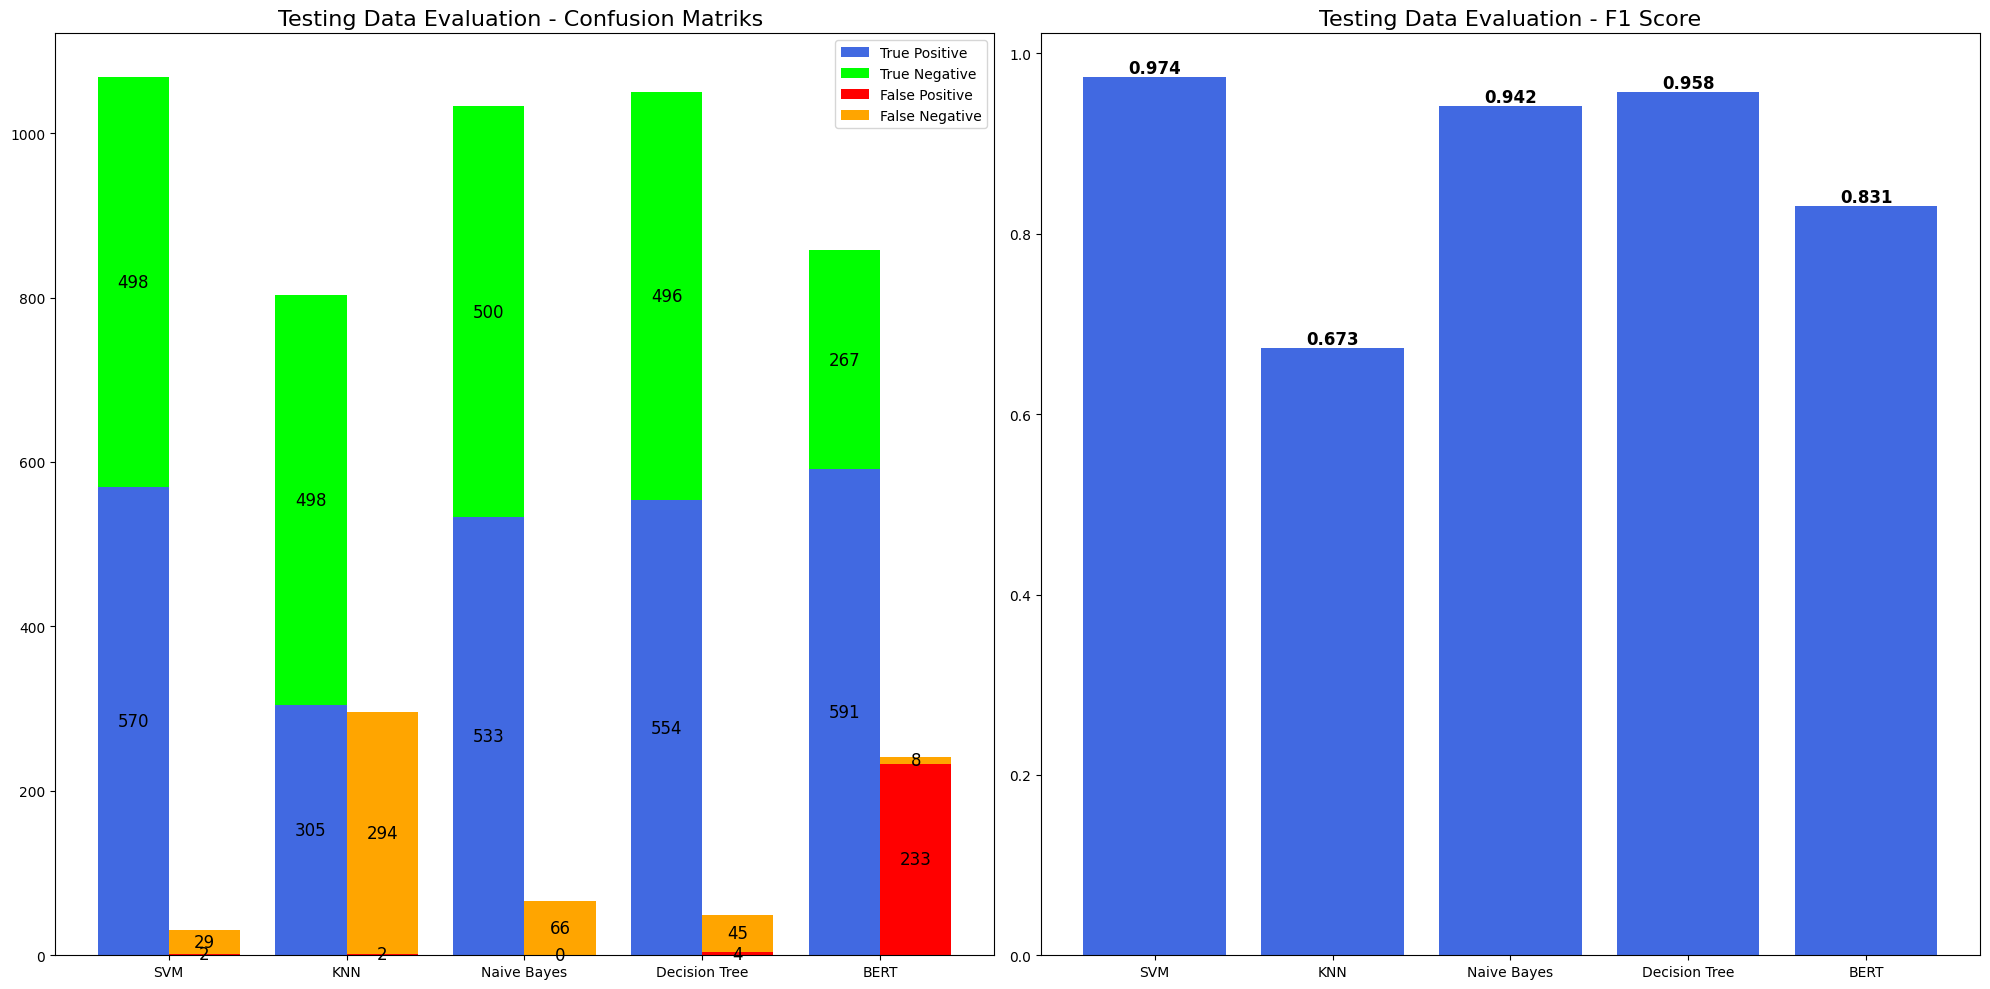
\includegraphics[width=1\linewidth]{img/f1score_test.png}
\caption{\label{fig:f1score_test}Perbandingan Confussion Matriks dan F1 Score antar model}
\end{figure}

\section{Conclusion}

Berdasarkan hasil penelitian yang telah dilakukan, dapat disimpulkan bahwa pendekatan supervised learning dengan delapan fitur yang telah dirancang oleh penelitian sebelumnya menunjukkan performa yang sangat baik dalam klasifikasi pasangan akronim dan ekspansi. Model Support Vector Machine (SVM) mendapatkan nilai F1-Score tertinggi sebesar 0,973 pada data testing, mengungguli model lainnya termasuk BERT yang memiliki F1-Score sebesar 0,830. Keunggulan ini menunjukkan bahwa fitur-fitur yang diekstraksi tersebut mampu menangkap karakteristik penting dari hubungan semantik antara akronim dan ekspansinya dengan efektif. Selain itu, stabilitas performa juga ditunjukkan oleh model Decision Tree dan Naive Bayes, meskipun masih berada di bawah SVM. Sebaliknya, K-Nearest Neighbor (KNN) dan BERT memiliki tantangan terutama dalam hal ketidakseimbangan antara precision dan recall, yang menyebabkan rendahnya F1-Score. Pada KNN, jumlah false negative yang tinggi menjadi faktor utama rendahnya recall, sedangkan pada BERT, jumlah false positive yang signifikan mengurangi precision.
Untuk penelitian selanjutnya dapat dilakukan kombinasi kedua pendekatan atau optimasi lebih lanjut pada preprocessing data dan fine-tuning model deep learning lainnya untuk menangkap pola atau karakteristik dari pasangan akronim dan ekspansi yang lebih akurat.



\bibliographystyle{plain}
\begin{thebibliography}{9}
\bibitem{ref1} Abidin TF, Mahazir A, Subianto M, Munadi K, Ferdhiana R. Recognizing Indonesian Acronym and Expansion Pairs with Supervised Learning and MapReduce. Information. 2020; 11(4):210.
\bibitem{ref2} Devlin, J. (2018). Bert: Pre-training of deep bidirectional transformers for language understanding. arXiv preprint arXiv:1810.04805.
\end{thebibliography}

\end{document}